%%%%%%%%%%%%%%%%%%%%%%%%%%%%%%%%%%%%%%%%%%%%%%%%%%%%%%%%%%%%%
%% global TEMPLATE (document class and untilites)
%%%%%%%%%%%%%%%%%%%%%%%%%%%%%%%%%%%%%%%%%%%%%%%%%%%%%%%%%%%%%
\RequirePackage{scrlfile}
\IfFileExists{template/hpi_thesis.cls}{
	\ReplaceClass{hpi_thesis}{template/hpi_thesis}
}{}
\documentclass{hpi_thesis}
%%%%%%%%%%%%%%%%%%%%%%%%%%%%%%%%%%%%%%%%%%%%%%%%%%%%%%%%%%%%%
%% HYPTHENATION
%%%%%%%%%%%%%%%%%%%%%%%%%%%%%%%%%%%%%%%%%%%%%%%%%%%%%%%%%%%%%

\hyphenation{Graph-struk-tur Story-patterns Story-pattern}



%%%%%%%%%%%%%%%%%%%%%%%%%%%%%%%%%%%%%%%%%%%%%%%%%%%%%%%%%%%%%
%% TODO MARKERS EETC
%%%%%%%%%%%%%%%%%%%%%%%%%%%%%%%%%%%%%%%%%%%%%%%%%%%%%%%%%%%%%

\newcommand{\citeNeeded}{\textcolor{hpired}{[citation~needed]}}
\newcommand{\factCheck}{\textcolor{hpired}{[check this fact]}}
\newcommand{\inlinetodo}{\textcolor{hpired}{ TODO HERE }}

\usepackage{framed, xcolor} 
\newcommand{\todo}[1]{
  \noindent \colorbox{lightgray}{\parbox{\textwidth}{
    \textcolor{black}{
      \large{ TODO: #1 }
    }
  }}
}
\newcommand{\note}[1]{
  \noindent \colorbox{lightgray}{\parbox{\textwidth}{
    \textcolor{black}{
      \small{ #1 }
    }
  }}
}
\newcommand{\question}[1]{
  \noindent \colorbox{hpired}{\parbox{\textwidth}{
    \textcolor{white}{
      QUESTION: #1 
    }
  }}
}
\newcommand{\answer}[1]{
  \noindent \colorbox{hpiyellow3}{\parbox{\textwidth}{
    \textcolor{black}{#1}
  }}
}
\newcommand{\todoExample}{
  \noindent \colorbox{hpiyellow3}{\parbox{\textwidth}{
    \textcolor{black}{
      \centerline{\large{ EXAMPLE HERE!}}
    }
  }}
}


\newcommand{\todoOptional}[1]{
  \noindent \colorbox{hpiyellow3}{\parbox[c][2cm]{\textwidth}{
    \textcolor{black}{ \large{OPTIONAL:~~ #1} }
  }}
}
\newcommand{\todoWrite}[1]{
  \noindent \colorbox{hpired3}{\parbox[c][2cm]{\textwidth}{
    \textcolor{black}{
      \centerline{\huge{ #1 } }
      \centerline{\large{...still needs major content!}}
    }
  }}
}
\newcommand{\todoImprove}[1]{
  \noindent \colorbox{hpiorange3}{\parbox[c][2cm]{\textwidth}{
    \textcolor{black}{
      \centerline{\huge{ #1 } }
      \centerline{\large{...still needs improvement / minor additions!}}
    }
  }}
}




%%%%%%%%%%%%%%%%%%%%%%%%%%%%%%%%%%%%%%%%%%%%%%%%%%%%%%%%%%%%%
%% OLD (giese template)
%%%%%%%%%%%%%%%%%%%%%%%%%%%%%%%%%%%%%%%%%%%%%%%%%%%%%%%%%%%%%

\newcommand{\appendixChapter}[1]{\chapter{#1}\setcounter{page}{1}}

\def\TReg{\textsuperscript{\textregistered}}

%\zitat{quotation}
\newcommand{\zitat}[1]{
 \begin{quote}
  \fboxsep5mm
  \shadowbox{
  \begin{minipage}{0.8\textwidth}
    #1
  \end{minipage}}
\end{quote}}

%\begriff{caption}{quotation or definition}
\newcommand{\begriff}[2]{
  \begin{quote}
  \fboxsep5mm
  \shadowbox{
  \begin{minipage}{0.8\textwidth}
   \begin{center}\textbf{#1}\end{center}
   \bigskip
   #2
  \end{minipage}}
  \end{quote}}

\definecolor{lightblue}{rgb}{0.9,0.9,0.9}
\definecolor{darkred}{rgb}{0.5,0,0}
\definecolor{darkgreen}{rgb}{0,0.5,0}
\definecolor{darkgrey}{rgb}{0.8,0.8,0.8}

\renewcommand*\lstlistingname{Quelltext}
%\JavaStyleBegin{title}{caption}{label}
\newcommand{\JavaStyleBegin}[3]{
  \begin{lstlisting}[language = Java,
   frame=none,
   framerule=1pt,
   tabsize=4,
   title={#1},
   caption={#2},
   label=#3,
   backgroundcolor=\color{lightblue},
   columns=fixed,
   basicstyle=\scriptsize \ttfamily \color{black},
   commentstyle=\itshape\color{darkgreen},
   keywordstyle=\bfseries\color{blue},
   stringstyle=\color{darkred},
   showspaces=false,
   breaklines=true,
   numbers=left,
   numberstyle=\tiny \color{magenta},
   showstringspaces=false,
   captionpos=b,
   xleftmargin=0.04\textwidth, 
   morekeywords={}]}
%\end{lstlisting}
																									
\newcommand{\methode}[1]{\sl #1\normalfont}
\newcommand{\klasse}[1]{\tt #1\normalfont}
\newcommand{\attribut}[1]{\textit{#1}}
\newcommand{\interface}[1]{\tt #1\normalfont}
\newcommand{\code}[1]{\ttfamily#1\normalfont}

\newcommand{\trenn}{\left|\right|}



\usepackage{pgfplots}
\pgfplotsset{width=7cm,compat=1.8}



%%%%%%%%%%%%%%%%%%%%%%%%%%%%%%%%%%%%%%%%%%%%%%%%%%%%%%%%%%%%%
%% document-specific data IMPORTS
%%%%%%%%%%%%%%%%%%%%%%%%%%%%%%%%%%%%%%%%%%%%%%%%%%%%%%%%%%%%%
\bibliography{content_extra/literature}
\loadglsentries{content_extra/glossary}

\makeglossaries
\newcommand{\docAuthor}{Arne Zerndt}
\newcommand{\docAuthorMail}{arne.zerndt@student.hpi.de}

\newcommand{\docTitleEn}{Supporting Iterative Development of Voice Interfaces using a Domain Specific Language}
\newcommand{\docTitleDe}{Unterstützen von Iterativer Entwicklung von Sprachassistenten durch einen Domänenspezifische Sprache}

\newcommand{\docCity}{Potsdam}
\newcommand{\docDate}{\today}

\newcommand{\docSupervisited}{Prof. Dr. Holger Giese}
\newcommand{\docChair}{System Analysis and Modeling Group}

\newcommand{\docIntituteShort}{Hasso Plattner Institute}
\newcommand{\docIntituteLong}{Hasso Plattner Institute for Digital Engineering}



%%%%%%%%%%%%%%%%%%%%%%%%%%%%%%%%%%%%%%%%%%%%%%%%%%%%%%%%%%%%%
%% MAIN DOCUMENT
%%%%%%%%%%%%%%%%%%%%%%%%%%%%%%%%%%%%%%%%%%%%%%%%%%%%%%%%%%%%%
\begin{document}
	\selectlanguage{english}

	%%% PDF-DOCUMENT-INFO
	\hypersetup{%
		pdftitle	= {\docTitleEn},
		pdfsubject	= {Bachelor's Thesis},
		pdfauthor	= {\docAuthor},
		pdfcreator	= {PDFLaTeX},
		pdfproducer	= {LaTeX with hyperref}		
	}
	
	
	
	%%%%%%%%%%%%%%%%%%%%%%%%%%%%%%%%%%%%%%%%%%%%%%%%%%%%%%%%%%%%%
	%% TITLEPAGE + PRE-CONTENT
	%%%%%%%%%%%%%%%%%%%%%%%%%%%%%%%%%%%%%%%%%%%%%%%%%%%%%%%%%%%%%
	\pagenumbering{Roman}
	\maketitle
	\cleardoublepage
	
	\chapter*{Abstract (English)}

This thesis seeks to address a current lack of version control systems for voice interface configurations. Instead of designing a new version control system for voice interface configurations, here a different solution is chosen. The voice interface configuration is adapted to fit into existing version control systems.
This is done by designing a domain specific language to describe the configuration of a voice interface in a text based way.
The voice interface technology chosen to demonstrate this solution is Google Dialogflow. The version control system chosen to focus on is Git, using Github.
For evaluation, an experiment with five test cases was conducted, comparing the domain specific language with the existing technology.
The results show a clear benefit in three of four criteria outlined, while maintaining parity in the fourth.
	\chapter*{Abstract (Deutsch)}

Diese Bachelorarbeit widmed sich einem derzeit bestehenden mangel an versionscontrollsystemen  für stimmliche benutzerschnittstellen.
Anstatt aber ein neues versionscontrollsystem für stimmliche benutzerschnittstellen zu bauen wird eine andere lösung gewählt. 
Eine stimmliche benutzerschnittstelle wird so adaptiert, dass sie mit bestehenden versionscontrollsystemen kompatibel ist.
Zu diesem  zweck wird eine domänenspezifische sprache entwickelt, die eine stimmliches benutzerschnittstelle auf eine textbasierten art spezifiziert. 
Um diese lösung zu demonstrieren wurde die sprach interface technologie Dialogflow gewählt, in verbindung mit dem versionscontrollsystem Git.
Für die Evaluation wurde ein experiment mit 5 test szenarien durgeführt, in dem die dömanenspzifische sprache mit der existierenden technologie verglichen wurde. Die ergebnisse zeigen einen klaren gewinn bei drei von vier zuvor spezifizierten kriterien, ohne verlust beim virten kriterium.


	\newpage
	\phantomsection
	\addcontentsline{toc}{chapter}{Table of Contents}
	\tableofcontents
 	
	
	%%%%%%%%%%%%%%%%%%%%%%%%%%%%%%%%%%%%%%%%%%%%%%%%%%%%%%%%%%%%%
	%% MAIN CONTENT
	%%%%%%%%%%%%%%%%%%%%%%%%%%%%%%%%%%%%%%%%%%%%%%%%%%%%%%%%%%%%%
	\cleardoublepage
	\pagenumbering{arabic}

	% ALL THE CHAPTERS
	
\chapter{Introduction}

The following Bachelor thesis is part of the "Ask your Repository!" Bachelor project.\footnote{\url{https://hpi.de/giese/lehre/bachelorprojekte/ask-your-repository.html}}\\
In this thesis, I will demonstrate a possible solution for the issue of synchronizing development on voice interfaces with that of application code by checking voice interface configuration into version control alongside the code it corresponds to. The focus will be on allowing the use of existing version control systems for voice interface configurations.\\
To approach this goal, I have designed a Domain Specific Language (DSL) to describe the configuration of a voice interface in a text-based but still abstract and intuitive way. \\
I will focus on development using Google Dialogflow as it is the most widely used tool \cite{Stackshare}; it is also what my Bachelor team is using in our project.
\footnote{The code for my DSL can be found here: \url{https://github.com/arne-z/BachelorThesis} and an implementation for the voice assistant in our bachelor project using the DSL can be found here: \url{https://github.com/hpi-sam/ask-your-repository-dialogflow-adapter/tree/agent-config-with-dsl}}

I propose that by designing a DSL that can be used to configure a Dialogflow agent in a way that is text based and can be managed by version control systems like Git - but that is intuitive to use for a developer familiar with the Dialogflow web interface -, development on voice interfaces can be simplified. Also, development teams in the future will be able to work on voice assistants in the same way that they are used to when working with code. This opens up the entirety of code based tools which exist for making development more streamlined for voice interfaces, while keeping the robustness of code which can be saved in version control.

In chapter 2, I will explain the current situation in regard to voice interface technology and version control. Afterwards, in chapter 3, I will specify the problem I am trying to solve in the thesis.
Chapter 4 will focus on finding a solution to the above mentioned problem, as well as on the specific solution I built a prototype for. Going into more detail, chapter 4.2 will show how I used Xtext to create a grammar and code generator for configuring Google Dialogflow agents. This grammar was used to provide syntax highlighting and validation in Eclipse DSL; the output of the code generator is a valid voice interface configuration in its JSON representation, ready to be imported into Google Dialogflow.
Lastly, in chapter 5 I will evaluate the success of the prototype by comparing it to an alternative way of checking voice interfaces into source control. 

\chapter{Status Quo}
\section{Voice Interfaces}
Voice interfaces, voice assistants, and chat bots are increasingly popular technologies \cite[page 8]{Olson2019} that are experimented with and used by every major player in the technology market \cite{Chatbots2018}. To keep up with this trend, developers either need to be able to build their own voice interfaces or integrate with an existing system of which there are many \cite{Alternativeto2019} and of which Google Assistant and Amazon Alexa are the most relevant; this can be seen in a survey Microsoft conducted this year on the popularity of voice assistants \cite[page 9]{Olson2019}.
Currently, depending on whether you are developing for Google Assistant or Alexa, designing a voice interface for one of these systems usually entails working with either Google Dialogflow or Amazon Lex. These are powerful tools which enable developers or domain specialists to quickly and easily design a voice interface.
These tools are interacted with through a website which provides a graphical editor for the configuration of the voice interface. 

\section{Version Control}
While the web interface makes initial setup of the voice interface easier for a single domain expert or developer, new difficulties arise when a team of developers is working on a voice interface in an iterative fashion. It becomes crucial for the team to manage versions and track changes to the interface along with the changes to the application the interface is supporting. 

As Martin Charles states in the text accompanying his Dialogflow CLI community tool \cite[page 1]{0xcaff2018}:
\zitat{
    DialogFlow stores intents and entities outside of source control. This makes rollbacks and keeping track of history difficult.
}
The state of the art solution for managing iterative work in development teams is Git. On GitHub alone there are more than 190 million Git repositories at present, as can bee seen by looking at \cite{Githuba}.
Git provides functionalities for saving snapshots of specific iteration in your project and handling the problems that come up in iterative work.\\
\begin{samepage}
    These problems are:
    \begin{itemize}
        \item merging work done by multiple developers
        \item ensuring that a stable version of a project is saved while developers are working on more experimental changes
        \item giving the team the ability to easily track and revert changes that have been made.
    \end{itemize}
\end{samepage}

The issue that arises is that the above mentioned technologies are not compatible and the configuration of a voice interface can easily get out of sync with the changes made to the application and managed in Git.

\chapter{Problem Statement}

As stated before, currently there is no version control system for Dialogflow agents.
This is problematic because when designing a voice interface, it is necessary to make iterative changes, so the voice interface can evolve alongside the application it supports. This can lead to issues in a number of different situation, and causes voice interface developers to miss out on the advantages modern software development gains from using Git.
\begin{itemize}
    \item When starting work on a new feature, a new branch is created. This is done so that changes, which might not work right away, are contained to this branch and can be merged into the main application at a later time. If this feature requires changes to the voice interface, a problem may arise, because the voice interface has no mechanism for branching.
    \item Once experimental changes on a feature branch advance to a point where they are meant to be included in the master branch, code can simply be merged from one branch to another. The changes to a voice interface configuration, however, cannot be included in a pull request.
    \item When working on a product, it is generally considered to be “best practice” to have code that should be merged into the master branch from a feature branch reviewed by at least one or two other developers to make sure that it is working as expected and does not have any obvious flaws. This cannot be done for changes to a voice interface.
    \item When working in a team, it is not always possible to remain aware of all the changes team members have made. Source code that is managed in Git automatically creates a history of all changes, which is highly valuable to the developers. This type of history does not exist for the voice interface configuration.
    \item Open source development is an important part of today's development landscape. Since voice interfaces are not usually checked into source control alongside application code, open source development of voice interfaces or applications that use voice interfaces is stifled. In addition, open source projects can be forked by other developers and can be improved by many developers in an iterative fashion. This is another advantage that voice interfaces are currently lacking. \\
    When working on a Dialogflow agent, one can save a version of the configuration and then continue as a draft, but Dialogflow assumes that you will only ever have one draft at a time. Versions are also designed in a linear fashion with no way to merge changes from multiple versions. This is obviously nowhere near the depth of features that are necessary in version control and all of these features are already provided for normal code by using the current state of the art version control system, Git.
\end{itemize}

In summary, the problem is that there is no sufficient version control system, that is compatible with Dialogflow.

\chapter{Approach}

\section{Choosing a Direction}

\subsection{Version Control System}

Since there is no version control system that is compatible with Dialogflow, the obvious solution might be to build a new version control system that is compatible with Dialogflow. This has been done before for other technologies.
An example of this would be the Open-source Version Control System for Machine Learning Projects that evolved from the neccessity of specialized version control for machine learning models and data sets.\cite{Petrov}\\
I decided against this approach for multiple reasons.

Firstly, I believe that it will be hard to get developers to move from an established tool like Git; I assume that developers would not choose to give up feature rich support that exists for Git (Github, Gitlab, Bitbucket to only name a few).
Secondly, using a specific version control system that is developed to allow compatibility with Dialogflow, it would be hard to also maintain compatibility with other tools.

Therefore, instead of trying and failing to develop a competing standard to Git, I decided to make use of a workaround that is possible with Dialogflow.

\subsection{Git with exported JSON files}

Another possibility would be to export a folder with a JSON representation of an agent and save this in Git. This solves some of the issues mentioned in chapter 3, but an agent's JSON representation is not intended for readability by humans, and neither is it meant for direct editing. This makes certain aspects of the workflows I described above much harder, e.g. conducting a code review, since it is difficult to read the changes to the JSON files describing the agent’s configuration.
This is the option currently used by many developers \cite{Oostinga} but that I decided against.\\
This is also the option that I will compare my prototype to in the evaluation chapter.

\subsection{Domain Specific Language}
While trying to solve the problems mentioned so far, it became obvious that a solution to these problems would require configuring an agent in a format that is compatible with text based tools like Git, but that also maintains or even enhances upon the maintainability and readability of Google Dialogflow configuration in the web interface.
For this purpose, I designed a domain specific language (DSL) in order to create a text-based notation (DSL code) for the configuration of an agent.

A solution like this has not been built for Dialogflow, most likely because voice interface tools like Amazon Lex or Google Dialogflow are a newer development, with Dialogflow having only existed in its current fashion since it's acquisition by Google at the end of 2016 \cite{Huffman2016} and the Dialogflow V2 API that I am using, and that was necessary for the success of this project currently being in Beta stage. The V2 API is generally available since April 2018 \cite{Imrie-Situnayake2018} and “V1 of Dialogflow´s API will be deprecated on October 23, 2019” \cite[page 1]{Dialogflow}.
Dialogflow is currently still transitioning to the use of the new V2 API.
It is the V2 API that makes this project possible because it includes the agent management APIs used for exporting, importing, and updating of Dialogflow agents \footnote{Agent is what Google calls a specific voice interface.} using the JSON format.


\section{DSL Engineering}


\subsection{What is a DSL?}

In contrast to a GPL (general purpose language), a DSL (domain specific language) is a smaller and more narrow programming language, and oftentimes is not Turing complete. The advantage of a DSL comes in the form of concise syntax, that is streamlined for one specific purpose. While a GPL has to allow the developer to be able to build quite literally anything within the constraints of the language, the DSL makes no such claims but can instead provide shortcuts for the few things that it is able to do. (Compare chapter 2 in \cite{Voelter2013}.)

I built a DSL prototype in Xtext using the Eclipse DSL language workbencH; it consists of two main parts.\\
Firstly, there is a grammar which defines all possible combinations of words that can be used to write in this language.
Specifying this grammar allows the developer to have live IDE support, including syntax validation, while writing DSL code.

The second part I built is a code generator.\\
This generator compiles DSL code into a collection of JSON files in a format accepted by the Google API. It allows the developer to automatically generate a working Dialogflow agent from their DSL code.

\subsection{Requirenments for the DSL}

In order to provide a tangible benefit, the DSL must fulfill a number of requirements:
\begin{itemize}
    \item It needs to be significantly shorter than the JSON representation of an agent.
    \item It needs to create smaller diffs\footnote{A diff refers to the sum of changed lines in a change.} than the JSON representation when making changes.
    \item It needs to be more readable than the JSON representation.
    \item A developer needs to be able to automatically compile and update an agent on the web from DSL code.
\end{itemize}

During the process of my work it became clear that solving the above mentioned problems made it necessary to find solutions for every one of these requirements.

\subsection{Design Decisions}

I wanted the DSL code to read naturally for a developer used to the Dialogflow interface.
In order to achieve this, I tried to closely mimic the structure of the web interface in my DSL code.

In order to show this, I will walk you through an example agent I created for testing purposes. The agent is a very simple controler for regulating the air conditioning in a room. It listens to the user and sends their requests to a server. Throughout the four steps of this example, I will follow a pattern of first showing how a developer would set up an agent on the Dialogflow website, followed by showing how to do the same in DSL code.

\subsubsection{Step 1: Creating an Agent}
First a developer needs to create a new agent. To do so, they click on "create agent" and enter the agent's name and language as seen in \autoref{CreateAgent}.
To achieve the same effect in DSL code, a developer would enter the following:
\begin{samepage}
    \begin{DSL}
        Agent TestAgent_RoomTemperature
            language en 
    \end{DSL}
\end{samepage}

\begin{figure}[!htb]
    \centering
    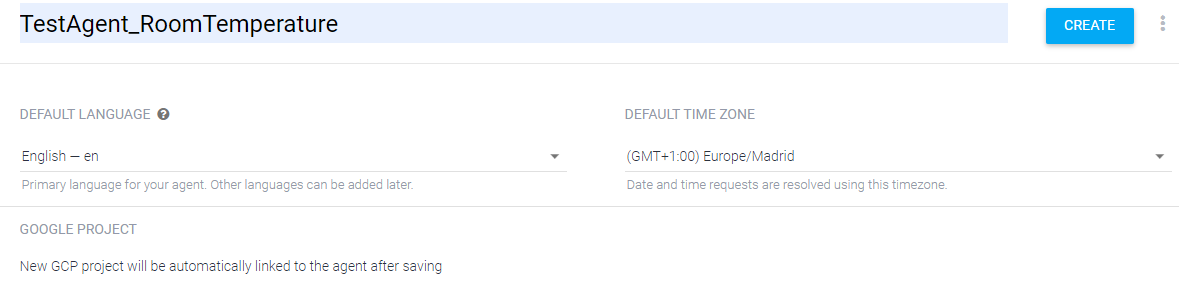
\includegraphics[width=1\textwidth]{Thesis_Images/CreateAgent.PNG}
    \caption{Creating an agent on Dialogflow.}
        \label{CreateAgent}
\end{figure}

\subsubsection{Step 2: Setting an Entity-Type}
In the next step, an entity-type needs to be created to allow to intuitively turn on and off the air conditioning.
In Dialogflow, this is achieved by filling in the form seen in \autoref{CreateType}.
In DSL code, the same can be done by writing the following:
\begin{samepage}    
    \begin{DSL}
        Agent TestAgent_RoomTemperature
            language en 
        
            Type ACState
                values 
                    "On" ("Active" "Enabled" "On"),
                    "Off" ("Inactive" "Disabled" "Off")
                auto_expand
    \end{DSL}
\end{samepage}

\begin{figure}[!htb]
    \centering
    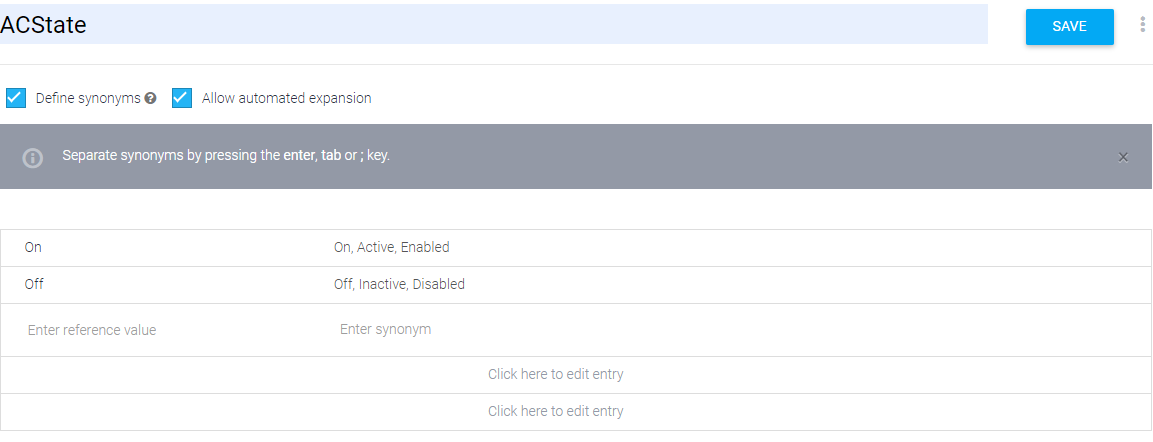
\includegraphics[width=1\textwidth]{Thesis_Images/CreateType.PNG}
    \caption{Creating an entity-type on Dialogflow.}
        \label{CreateType}
\end{figure}

\subsubsection{Step 3: Setting a Webhook}
For the agent to actually affect an air conditioner in the real world, it needs to send the user's request to a webserver. To do so, a webhook is enabled in Dialogflow by filling in the form as seen in \autoref{CreateWebhook}.
In DSL code, the same can be achieved:
\begin{samepage}
    \begin{DSL}
    Agent TestAgent_RoomTemperature
        language en 
            
        Webhook 
            active 
            url "https://fake.ac_controller.com/vi_webhook"

        Type ACState
            values 
                "Off" ("Inactive" "Disabled" "Off"),
                "On" ("Active" "Enabled" "On")
            auto_expand
    \end{DSL}
\end{samepage}

\begin{figure}[!htb]
    \centering
    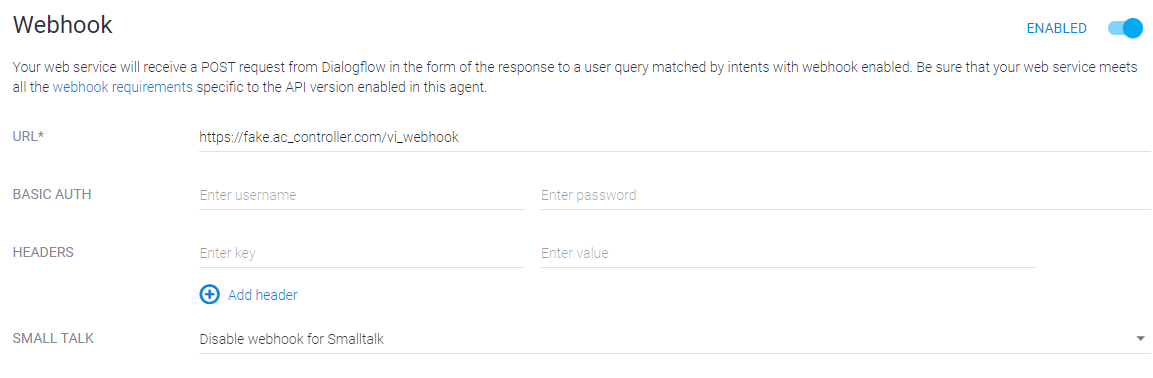
\includegraphics[width=1\textwidth]{Thesis_Images/CreateWebhook.PNG}
    \caption{Setting a webhook on Dialogflow.}
        \label{CreateWebhook}
\end{figure}

\subsubsection{Step 4: Writing an Intent}

The last and most vital step is to create an intent that the agent can understand. This is done on the website by filling in the form seen in \autoref{CreateIntent} and can alternatively be achieved in DSL code as follows:

\begin{figure}[!htb]
    \centering
    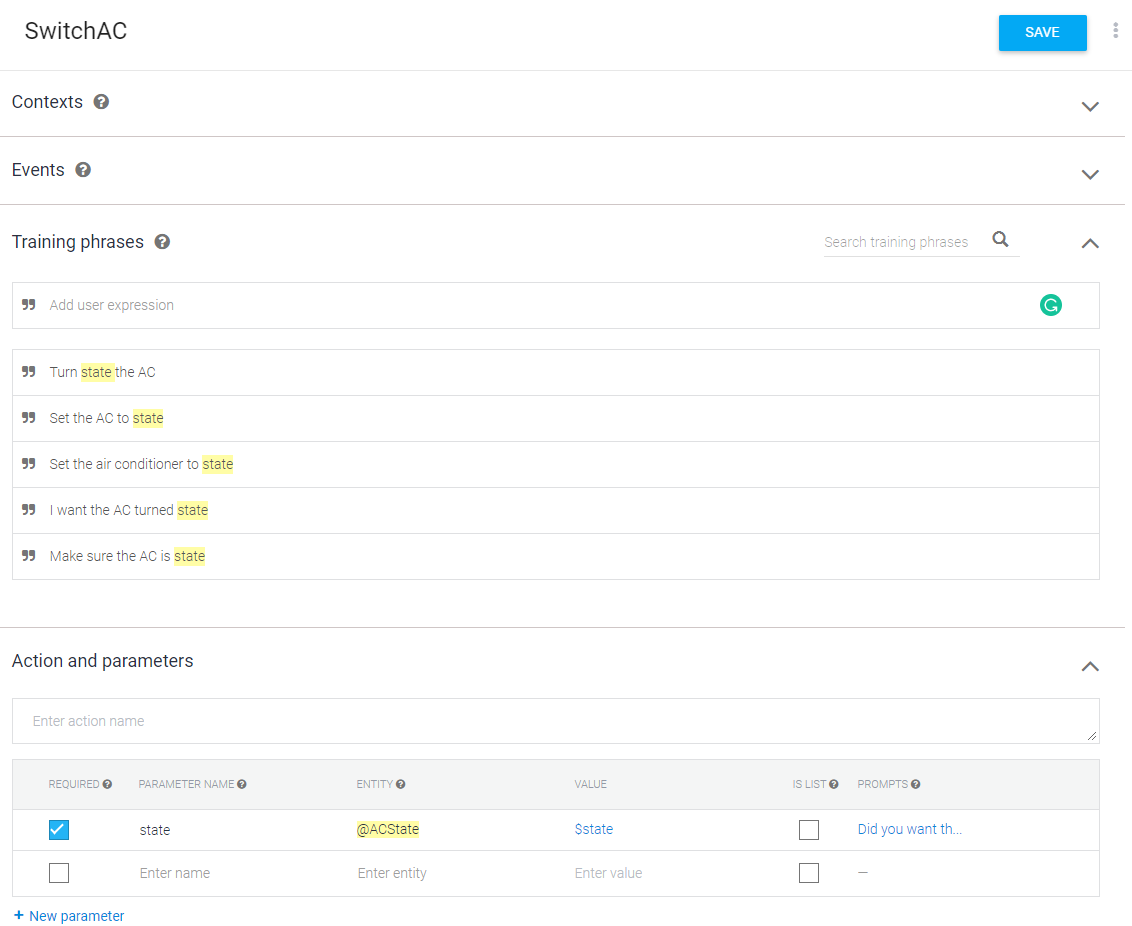
\includegraphics[width=1\textwidth]{Thesis_Images/CreateIntent.PNG}
    \caption{Setting up an intent on Dialogflow.}
        \label{CreateIntent}
\end{figure}
\begin{samepage}
    \begin{DSL}
        Agent TestAgent_RoomTemperature
            language en 
                
            Webhook 
                active 
                url "https://fake.ac_controller.com/vi_webhook"

            Type ACState
                values 
                    "Off" ("Inactive" "Disabled" "Off"),
                    "On" ("Active" "Enabled" "On")
                auto_expand

            Intent SwitchAC
                parameters
                    state ACState (required prompts 
                        "Did you want the AC turned On or Off?")
                trained with phrase
                    "Turn" state "the AC",
                    "Set the AC to" state,
                    "Set the air conditioner to" state,
                    "I want the AC turned" state,
                    "Make sure the AC is" state
                webhook_fullfillment
    \end{DSL}
\end{samepage}

\subsection{Usage}

When developing with the DSL I designed, in order to update the Dialogflow agent on the web, you run the compiler for the DSL using the DSL code as input; the output will be a full JSON representation of the Dialogflow agent which can be sent to the Dialogflow V2API.
The V2API allows you to update the online version of your agent using the JSON files. For this you can either use the Dialogflow-Cli tool \cite{0xcaff2018} the Dialogflow comunity has built, or build your own script like I did.

\subsection{Dynamic Entity Control}

In our Bachelor project, we have some entity types that are dynamically updated via the Dialogflow API, in order to stay up to date with our production database. For example, we have the team entity type, that is populated with the names of teams that are signed up to our service. This allows a user to select his team via the voice assistant.
Since teams are created and deleted by the users, we need to update the entity type while the service is deployed.
This makes it impossible to have a list of all teams written down in the DSL code to send to the server. 
To make this possible I added the keyword “dynamic” for an entity type in the DSL I designed.
This keyword allows the developer to have the type exist in the DSL and be valid for syntax validation - but not have any JSON files generated for it, so as not to overwrite an entity type that is dynamically set on Dialogflow via the API.

\section{Target Group}

If you are a small group under time pressure, and you do not need to maintain the agent throughout it's co-evolution with your application, continuing to use the Dialogflow web interface will be simpler than adopting the DSL I wrote.

However, this DSL is directed at teams of developers who will be working on an agent for an extended time, and for whom using version control is a neccessity.
I expect that the group of developers who will be most interested in this DSL will be those, who are currently using the approach of saving the JSON  version of their agent in source control.
These developers will find advantages in multiple points that I will discuss in the next chapter.

\chapter{Evaluation}
In the following chapter I will evaluate the performance of my DSL-prototype.
Testing and evaluation have been done by me, referring back to the requirements I stated earlier in chapter four. A future larger scale survey would be welcome but was not part of this evaluation.\\
The categories I used for evaluation were:
\begin{itemize}
    \item length
    \item diff size
    \item readability
    \item automatic compilation and update
\end{itemize}

In the following sections I will introduce each of these categories and how the DSL prototype compares to the existing technology referring to each of them.

\section{Length}

In order to provide a tangible benefit, the DSL code must be significantly shorter than the JSON representation. Coming back to the test case agent used in chapter four, I can show that the DSL code for that agent is exactly 23 lines long, three of which are left blank for better readability (see \autoref{RoomTemperature Agent DSL}).
The JSON version for this same agent, however, comes in at exactly 200 lines (see \autoref{RoomTemperature Agent JSON}) meaning it is almost ten times as long. This is a trend that continues accross all my five test cases, as can be seen in \autoref{SizeChart}.

\begin{figure}
    \centering
    \caption{Test Cases: difference in configuration size}
    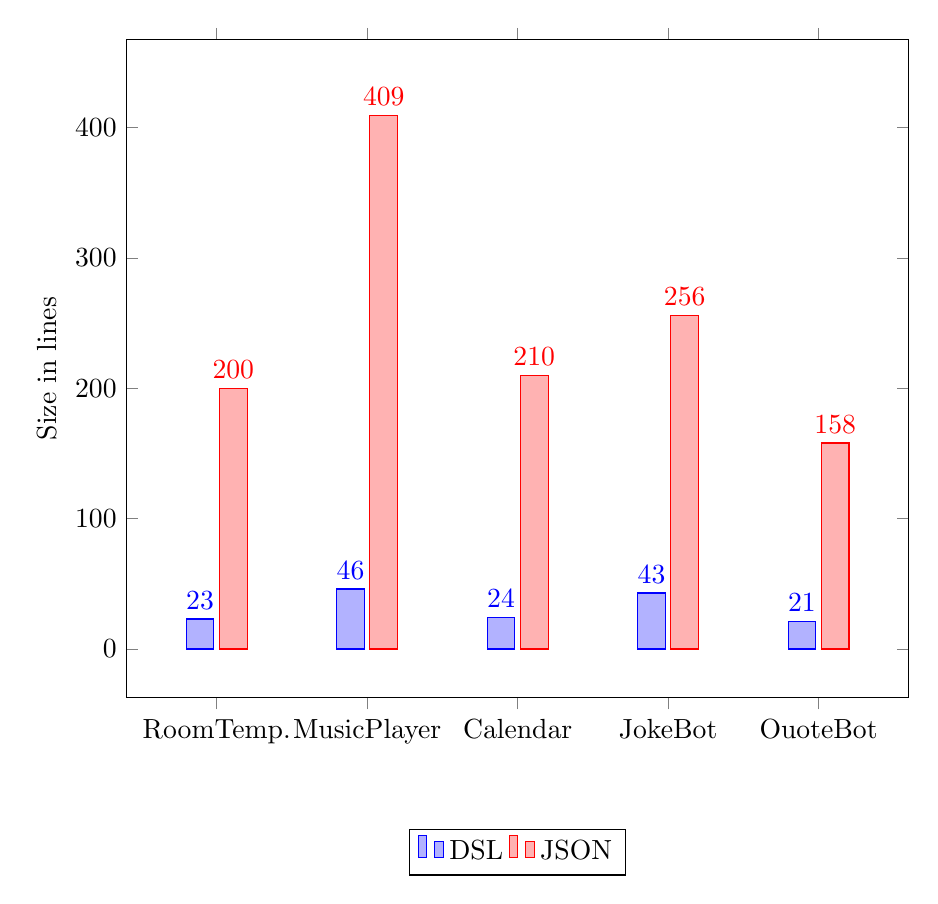
\begin{tikzpicture}
        
        \begin{axis}[
            ybar,
            width=0.95\textwidth,
            enlargelimits=0.15,
            legend style={at={(0.5,-0.2)},
              anchor=north,legend columns=-1},
            ylabel={Size in lines},
            symbolic x coords={RoomTemp., MusicPlayer, Calendar, JokeBot, OuoteBot},
            xtick=data,
            nodes near coords,
            nodes near coords align={vertical},
            ]
        \addplot coordinates {(RoomTemp.,23) (MusicPlayer, 46) (Calendar,24) (JokeBot,43)  (OuoteBot, 21)};
        \addplot coordinates {(RoomTemp.,200) (MusicPlayer, 409) (Calendar,210) (JokeBot,256) (OuoteBot, 158)};
        \legend{DSL,JSON}
        \end{axis}
    \end{tikzpicture}
    
    \label{SizeChart}
    
\end{figure}

This demonstrates that the DSL code for an agent is significantly shorter than the JSON version which saves the developer valuable time, e.g. when conducting a code review. This is a large benefit in and of itself, but it is amplified by the following point.


\section{Diff Size}
It is non length alone, but the DSL code must also create smaller diffs\footnote{A diff refers to the sum of changed lines in a change.} than the JSON representation when making changes.

Using the air conditioning example again, when making a change - in this case adding more training phrases to an agent to allow additional functionality - the diff size shows a large difference between DSL code and JSON version. In this specific example, the DSL code has a diff of 7 lines (as seen in \autoref{RoomTemperature Agent DSLDiff}) and the JSON version one of 124 lines (see \autoref{RoomTemperature Agent JSONDiff}).
An overview of all test cases is given in \autoref{DiffChart}.

It is also noteworthy that the DSL code causes less unintended diffs, as some elements of the JSON - like generated Unique Identifiers - can cause diffs that are unrelated to any intentional changes by the developer (as seen in \autoref{RoomTemperature Agent JSONDiff}).

\begin{figure}
    \centering
    \caption{Test Cases: difference in diff size.}
    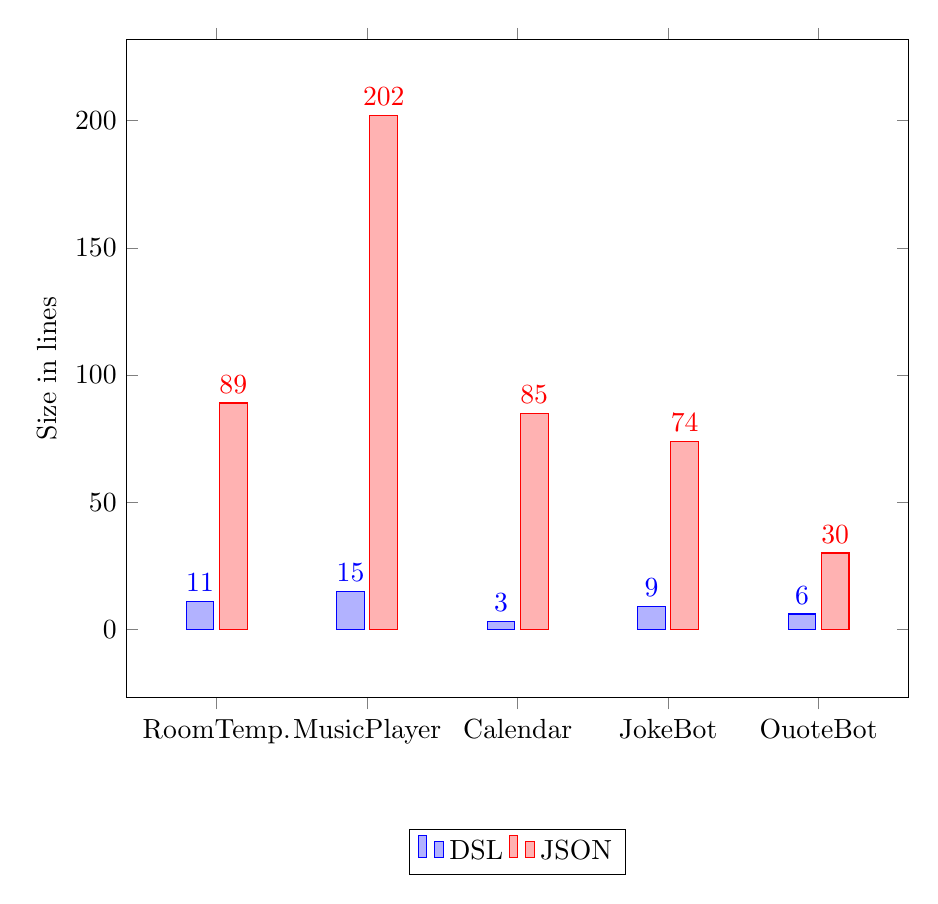
\begin{tikzpicture}
        \begin{axis}[
            ybar,
            width=0.95\textwidth,
            enlargelimits=0.15,
            legend style={at={(0.5,-0.2)},
              anchor=north,legend columns=-1},
            ylabel={Size in lines},
            symbolic x coords={RoomTemp., MusicPlayer, Calendar, JokeBot, OuoteBot},
            xtick=data,
            nodes near coords,
            nodes near coords align={vertical},
            ]
        \addplot coordinates {(RoomTemp.,11) (MusicPlayer, 15) (Calendar,3) (JokeBot,9) (OuoteBot, 6)};
        \addplot coordinates {(RoomTemp.,89) (MusicPlayer, 202) (Calendar,85) (JokeBot,74)(OuoteBot, 30)};
        \legend{DSL,JSON}
        \end{axis}
    \end{tikzpicture}
    
    \label{DiffChart}
    
\end{figure}

\section{Readability}

While length is an objective criterion, readability is innately more subjective, as it relates to how well a developer will be able to understand a piece of code.\\
For this comparison I will focus on five criteria; the first three are reworded from developer Egon Elbre's article "The psychology of code readability" \cite{Elbre}; the last two are based on my own observations.
\begin{itemize}
    \item Cohesive pieces of code conveying one idea at a time.
    \item Descriptive - but not overly long - names and keywords.
    \item Using idioms from natural language.
    \item Indentation and whitespace.
    \item Leaving out unneccessary values.
\end{itemize}

\subsubsection{Cohesive pieces of code conveying one idea at a time}

The following piece of JSON configuration defines a single training phrase for the SwitchAC intent, from the same example used above. The intent itself is not defined in the same file, since training phrases are kept in a seperate file in the JSON configuration.
\begin{samepage}
    \begin{JSON}
        {
            "id": "ed813a56-e6e9-4bce-b0ed-dca488102333",
            "data": [
              {
                "text": "Turn ",
                "userDefined": false
              },
              {
                "text": "state ",
                "alias": "state",
                "meta": "@ACState",
                "userDefined": true
              },
              {
                "text": "the AC ",
                "userDefined": false
              }
            ],
            "isTemplate": false,
            "count": 0,
            "updated": 1560083189
          },
    \end{JSON}
\end{samepage}

This is equivalent to the following lines found in my SwitchAC example:
\begin{DSL}
    trained with phrase
        "Turn" state "the AC"
\end{DSL}
As can clearly be seen, the JSON configuration is intended for automatic parsing, rather than for human readability. It is also limited by the key value and stringly typed nature of the configuration in JSON format. In my DSL, the training phrase can easily be traced back to it's intent, which is defined just three lines above in the room temperature example.

\subsubsection{Descriptive - but not overly long - names and keywords}

I chose all the keywords in my DSL to read like they would on the Dialogflow website.
This means that setting a new intent uses the keyword "Intent", defining a parameter for the intent uses the "parameters" keyword, and contexts are managed be using the "contexts" keyword - followed by either "input" or "output", depending on whether input or output contexts are set.

In contrast, the JSON example I showed above contains keys with names like "data" for a training phrase, "meta" for the type a parameter corresponds to, and the "isTemplate" key which is always set to false, because it is depracated.

\subsubsection{Using idioms from natural language}

When designing the syntax for my DSL, I tried - whenever possible - to use syntax that reads like a normal sentence in natural language. This is why a developer writes: 
\begin{DSL}
    trained with file
        "filename"
\end{DSL}
in order to include a file with pre-generated training phrases. A reader can immediately understand what the otherwise not always recognizable filename refers to.

In contrast, the JSON representation is modeled after the structure of a JavaScript object and is meant to accurately describe objects and their attributes in computer progams. It does not use idioms from natural language to attempt intuitive understanding of an agent's behaviour.
A specific advantage of the DSL version is that it was designed from the beginning to intuitively convey agent behaviour.

An example worth mentioning here is the definition of a fallback intent, which is an intent only used if no other intent can match the user's utterance.
In the JSON representation a fallback intent is only different from a regular intent by a boolean value at the very bottom of the intent description:
\begin{JSON}
    "fallbackIntent": true,
\end{JSON}
This works perfectly fine if the intention is for the file to be parsed by a computer, but for human readability, the way the Dialogflow website handles this is much more beneficial.
On the website a fallback intent is visually distinguished from normal intents and is created with a separate button.
For the DSL version, I decided that a fallback intent should be defined as follows:
\begin{DSL}
    fallback Intent DefaultFallbackIntent
        response 
            "I didn\u0027t get that. Can you say it again?"
            "I missed what you said. What was that?"
            "Sorry, could you say that again?"
            "Sorry, can you say that again?"
            "Can you say that again?"
            "Sorry, I didn\u0027t get that. Can you rephrase?"
            "Sorry, what was that?"
            "One more time?"
            "What was that?"
            "Say that one more time?"
            "I didn\u0027t get that. Can you repeat?"
            "I missed that, say that again?"
        action 'input.unknown'
\end{DSL}
This example is the default fallback intent that every agent on the Dialogflow website is created with. Note that the definition begins with \textit{fallback Intent} instead of \textit{Intent}. This immediately makes it clear to the reader that this intent should be read as a fallback and not as a regular intent.

\subsubsection{Indentation and whitespace}

An additional benefit for readability is the ability to seperate a program into meaningful paragraphs.

This can be seen in \autoref{RoomTemperature Agent DSL}, where between each instruction I left a blank line. This helps visually seperate the code into meaningful units.

As a further project, but not possible in the scope of this thesis, an automatic linting and formating tool for the DSL could be considered. Similar tools have been developed for general programming languages numerous times with a very popular example being Black for Python \cite{Python} and numerous other examples existing \cite{Github}.

\subsubsection{Leaving out unneccessary values}

One of the most important ways of reducing clutter in the agent configuration - and of thereby reducing the configuration's size - is to leave out unneccessary values like unchanged default values and empty values.
If an agent does not have a description, the JSON representation will carry the following line.
\begin{JSON}
    "description": "",
\end{JSON}
Instead, the DSL version simply will not have a line concerning the description, since it is not changed from it's default value of being an empty string.
The same is done for a large number of settings that a developer is able to change in DSL code but that have a default value in Dialogflow. They need not be displayed in DSL code if the default value is not changed.


\section{Automatic compilation and update}
A developer needs to be able to automatically compile and update an agent on the web from DSL code.
The compiler created alongside this prototype\footnote{\url{https://github.com/arne-z/BachelorThesis/releases}} is able to automatically generate the JSON representation of an agent from DSL code.
Alongside this, I have written a script that automatically sends the resulting JSON files to the Dialogflow website.
This can be used in continuous integration setups like CircleCI \cite{CircleCI} to automatically keep the online version of a Dialogflow agent up to date with the most current version of the DSL code in source control.

Below, you can see an example of the CircleCI job configuration that I set up for the prototype in our Bachelor project.
\footnote{The full configuration set up by our Bachelor project team can be found here:\\
\url{https://github.com/hpi-sam/ask-your-repository-dialogflow-adapter/blob/agent-config-with-dsl/.circleci/config.yml}}
\begin{samepage}    
    \begin{lstlisting}
        deploy_agent:
            docker:
                - image: circleci/openjdk:latest-node
            steps:
                - checkout
                - run: > 
                    wget -O ./dfc_compiler.jar
                    https://github.com/arne-z/BachelorThesis/...
                - run: yarn install
                - run: > java -jar ./dfc_compiler.jar 
                    ./Agent/Tobito.dfc
                - run: > echo $GOOGLE_CERT_FILE_64 
                    | base64 --decode > ./googleKey.json
                - run: >
                    node ./utility/importAgent.js 
                    --dir ./src-gen 
                    --key ./googleKey.json 
                    --pid projects/newagent-bdb60
    \end{lstlisting}
\end{samepage}

The above configuration starts a docker image with Java and Node installed - Java is required for the DSL compiler, Node for the import script - and checks out the most recent version of our project from source control.
It then downloads the DSL compiler from my github repository and runs the compiler targeting the .dfc file containing the DSL code for our project's agent.
Afterwards, it runs the importAgent script that will send the JSONs generated by the compiler to the Dialogflow API.

This setup allows a "hands free" approach to developing for Dialogflow, where all the developer has to do is change the DSL code; once that is pushed to Git, the Dialogflow agent is updated automatically.


\section{Concessions and Drawbacks}

Working with the DSL instead of Dialogflow directly comes with some drawbacks, as I had to make certain concessions during development. 
These concessions can be divided into four categories.

\subsection{Design Choices differing from the Dialogflow Website}
As I stated before, I attempted to stay as close to the Dialogflow website as possible, but there are some elements of the website that do not lend themselves to being translated into a text based configuration.

The way parameters are entered in Dialogflow is an interesting example of this, as is shown in \autoref{CreateIntent}. Translating to a text based interface with the requirement of live syntax validation, it became neccessary to enter the parameters allowed in training phrases before defining the phrases.
Similarly, Dialogflow switched from what is called \textit{template mode}, where a training phrase would be described as, e.g.: "Turn state the AC", to what is called \textit{example mode}, which means the phrase would be: "Turn on the AC" - with the "on" being annotated to show that it is meant to represent a number of possible values.
In order to translate this to a text based interface, I considered a solution that would have looked as follows:

\begin{DSL}
    Intent SampleIntent
        trained with phrase
            "Turn {on : state} the AC"
\end{DSL}

I eventually decided against this, as I perceived this solution to make both writing and reading the training phrases unneccessarily difficult. Instead I decided to continue using the template format for the DSL as seen below:

\begin{DSL}
    Intent SampleIntent
        trained with phrase
            "Turn" state "the AC"
\end{DSL}

This works and is fairly easy to read but is still a compromise and doesn't quite allow the same user experience as the Dialogflow website.

\subsection{The Difficulty of Deciding on Defaults.}

A large part of what makes both the web interface and the DSL easier to work with than the JSON files, is that here a developer can assume all the defaults to be reasonable. When first creating a new Dialogflow agent, all the default settings are already set for you to start working with. I found that for my tool I was able to use the same defaults that the website uses, so that the same workflow of creating an agent arrives at the same results on the website and in the DSL.

This lead to a bit of a problem when it came to the two default intents that a Dialogflow agent is created with, the "Default Fallback Intent" and the "Default Welcome Intent". \\
I considered adding these default intents during compilation, unless the developer specifically disabled this, but I found that to be too unintuitive. On the Dialogflow website, a developer can always see the list of intents in the agent, including these two default intents on the intents panel, but in a text based interface the developer cannot easily be informed of the default intents existing in the background. Instead, I decided that only the intents described in the developer's code should be in the compiled agent. \\
My plan is to add a shortcut for enabling the default intents via a \textbf{use\_default\_intents} flag, so that the developer can easily use the default intents, and anyone reading the code will still know these intents are enabled.

\subsection{Unsupported Dialogflow Features}

Dialogflow is a large project, much bigger in scope than this thesis, so it was immediately apparent that my prototype would not be able to support all of the features and settings that are available in Dialogflow.
Instead, I selected the features that were neccessary to support developemt in my Bachelor project.
This means that some projects might be unable to use this prototype, as they rely on features that are not supported.


\chapter{Summary and further Work}

It was my self-set task for this Bachelor thesis to find a solution for shortcomings in available version control for Dialogflow agents. In order to accomplish this, I built a prototype of a DSL for describing Dialogflow agents.
When starting this project my assumption was, that there should and could be a solution for using version control with a Dialogflow agent that is simpler, shorter, and more readable than saving the JSON cofiguration of the agent in source control.\\
The solution I eventually built is aimed at teams of developers working longer term on maintaining an agent throughout it's coevolution with their application.
I arrived at this solution because, from the very beginning, I wanted to find a way for developers to work with dialogflow without leaving their familiar way of working.\\
In order to build this DSL, I had to design a grammar to describe the syntax possible in the language and build a code generator using this grammar to generate JSON files.\\
In order to test and evaluate this prototype, I designed five test cases in each of which I compared the performance of the prototype with that of the established way of saving the agent configuration using JSON files.\\
In result, I have found that the DSL provides a measurable improvement in both the size of agent configurations and the size of diffs created by changes to the configuration - to be more precise: a 87.15\% reduction in size and a 88.9\% reduction in diff size on average respectively (see \autoref{ResultTables}) - while also improving readability and almost entirely maintaining the ease of updating the agent's online version.\\
Teams working with this tool will find that it offers benefits in regard to teamwork, learning, consistency, and keeping track of their version history.
The code for my prototype is available online, free and open source.

There are a number of questions still unanswered, and as I mentioned above, some improvements to the DSL are still possible.
Some further projects one could consider are:
\begin{itemize}
    \item A larger survey for better evaluation of long term benefits to teams working with this tool.
    \item Finding out whether it is possible to use a DSL like this to create agents in a uniform language for both Dialogflow and Amazon Lex.
    \item Build a production-ready tool from the prototype that achieves full feature parity with the Dialogflow web interface.
    \item Build a generator for DSL code from Dialogflow JSON exports, to help teams reduce the cost of switching to the DSL solution.
\end{itemize}

For the nearest future, my tool will help my Bachelor project team with working on our own Dialogflow agent.


	%%%%%%%%%%%%%%%%%%%%%%%%%%%%%%%%%%%%%%%%%%%%%%%%%%%%%%%%%%%%%
	%% APPENDIX
	%%%%%%%%%%%%%%%%%%%%%%%%%%%%%%%%%%%%%%%%%%%%%%%%%%%%%%%%%%%%%
	\cleardoublepage
	% \pagenumbering{Roman}
	\appendix

	% ALL APPENDIX STUFF
	\printbibliography[heading=bibintoc]
	\clearpage
	\chapter{Declaration of Authorship} 

\section*{Declaration} 

I hereby declare that the thesis submitted is my own unaided work and that I did not use any other sources and aids than those referenced.
% All direct or indirect sources used are acknowledged as references.

\bigskip\bigskip

\section*{Eidesstattliche Erklärung}
\selectlanguage{ngerman}

Ich erkläre hiermit, dass ich die vorliegende Arbeit selbstständig verfasst und dafür keine anderen als die genannten Quellen und Hilfsmittel verwendet habe.
% Die aus fremden Quellen direkt und indirekt übernommenen Gedanken sind als solche kenntlich gemacht. 

\bigskip\bigskip\bigskip\bigskip



\begin{minipage}{6cm}
\docCity{}, den \docDate
\bigskip\bigskip\bigskip


\hrulefill

\small{\docAuthor}
\end{minipage}
	\chapter{DSL Code of Test Agents}
The following examples are in some cases formated differently from the way they were during my tests, leading to slightly differing line numbers. They were reformated to fit into the printed version. Original files can be found on my GitHub.\footnote{\url{https://github.com/arne-z/BachelorThesis/tree/master/dsl_code}}

\section{RoomTemperature Agent}
\label{RoomTemperature Agent DSL}

\begin{lstlisting}
Agent TestAgent_RoomTemperature
  language en 
    
  Webhook 
    active 
    url "https://fake.ac_controller.com/vi_webhook"

  Type ACState
    values 
      "Off" ("Inactive" "Disabled" "Off"),
      "On" ("Active" "Enabled" "On")
  auto_expand

  Intent SwitchAC
    parameters
      state ACState (required prompts
        "Did you want the AC turned On or Off?")
    trained with phrase
      "Turn" state "the AC",
      "Set the AC to" state,
      "Set the air conditioner to" state,
      "I want the AC turned" state,
      "Make sure the AC is" state
    webhook_fullfillment
\end{lstlisting}

\pagebreak

\section{MusicPlayer Agent}
\label{MusicPlayer Agent DSL}

\begin{lstlisting}
Agent MusicPlayer
  language en
  
  Webhook
    active
    url "https://fake.music_controller.com/vi_webhook"
    
  Intent PlaySong
    parameters 
      Artist music_artist
      Genre music_genre
      Title any
    trained with phrase
      "Play a " Genre "song",
      "Play some" Genre,
      "Play a song by "Artist,
      "Play" Title "by" Artist,
      "Play" Title,
      "Play a random song"
    webhook_fullfillment
    
    Intent StopMusic
      action "StopMusic"
      trained with phrase
        "Pause",
        "Stop",
        "Quiet",
        "Stop the Music"
      webhook_fullfillment
    
    Intent VolUp
      action "VolUp"
      trained with phrase
        "Louder",
        "More Volume",
        "Too quiet",
        "Volume Up"
      webhook_fullfillment
      
    Intent VolDown
      action "VolDown"
      trained with phrase
        "Lower Volume",
        "Too loud",
        "Volume Down"
      webhook_fullfillment
\end{lstlisting}
\pagebreak


\section{Calendar Agent}
\label{Calendar Agent DSL}

\begin{lstlisting}
Agent Calendar
  language en

  Webhook
    active
    url "https://fake.calendar_controller.com/vi_webhook"
  
  Type Entry
    values 
      "Appointment", 
      "Reminder", 
      "Event"
    auto_expand
  
  Intent AddEntry
    parameters 
      Entry Entry
      Time date_time (required prompts "For when should I
        enter that entry?")
      Title any (required prompts "What should I call the entry?")
    trained with phrase
      "Add a new" Entry "for" Time,
      "Add a new" Entry,
      "Add a" Entry "at" Time Title
    webhook_fullfillment
\end{lstlisting}
\pagebreak


\section{JokeBot Agent}
\label{JokeBot Agent DSL}

\begin{lstlisting}
Agent JokeBot
  language en
  
  Webhook
    active
    url "https://fake.rate_my_jokes.com/vi_webhook"
  
  Intent DadJoke
    contexts 
      output joke 
    trained with phrase
      "Tell me a Dad joke",
      "Do you know any stupid jokes?",
      "Do you know any dad jokes?"
    response 
      "What is brown and sticky? ... A stick."
      "My wife is really mad at the fact that I have no
        sense of direction. So I packed up my stuff and right."
      "I bought some shoes from a drug dealer. I don't know what
        he laced them with, but I was tripping all day!"
      "Why can't you hear a pterodactyl go to the bathroom?
        Because the pee is silent."
  
  Intent RateJokePositive
    contexts 
      input joke
    action "ratePositive"
    trained with phrase
      "Wow that was funny",
      "That was awesome",
      "I liked that joke"
    response
      "Glad you liked it."
    webhook_fullfillment
  
  Intent RateJokeNegative
    contexts 
      input joke
    action "rateNegative"
    trained with phrase
      "Bad joke",
      "Don't tell that joke again",
      "Thanks, I hate it."
    response
      "Well that's your loss, I like the Joke."
    webhook_fullfillment
\end{lstlisting}
\pagebreak


\section{QuoteBot Agent}
\label{QuoteBot Agent DSL}

\begin{lstlisting}
Agent QuoteBot
  language en
  
  Intent OscarWildeQuote
    trained with phrase
      "Tell me a quote by Oscar Wilde",
      "What would Oscar Wilde say"
    response
      "To live is the rarest thing in the world. 
        Most people exist, that is all."
      "Only dull people are brilliant at breakfast."
      "I think God, in creating man,
        somewhat overestimated his ability."
      "Democracy means simply the bludgeoning of the people
        by the people for the people."
      
  Intent EinsteinQuote
    trained with phrase
      "Tell me a quote by Albert Einstein",
      "What would Einstein say"
    response
      "Two things are infinite: the universe and
        human stupidity; and I'm not sure about the universe."
      "If you can't explain it to a six year old,
        you don't understand it yourself."
      "Never memorize something that you can look up."
\end{lstlisting}
	\chapter{Examples of Diffs created from Test Agents}

\section{RoomTemperature Agent}
\label{RoomTemperature Agent DSLDiff}

\begin{lstlisting}
  @@ -26,9 +26,14 @@ Agent TestAgent_RoomTemperature
     Intent ChangeTemperature
       parameters 
         temp temperature (required prompts "What temperature 
           would you like the AC set to?")
  +      point time
       trained with phrase 
         "Set the AC to" temp, 
         "Set the air conditioner to" temp, 
         "I want the AC turned to" temp, 
  -      "Make sure the AC is at" temp
  +      "Make sure the AC is at" temp,
  +      "Set the AC to" temp "at" point, 
  +      "Set the air conditioner to" temp "at" point,
  +      "I want the AC turned to" temp "at" point,
  +      "Make sure the AC is at" temp "at" point
       webhook_fullfillment
\end{lstlisting}

\section{Test Agents 2-5}
The diffs created from the other four test agents are not printed here to prevent the appendix from becoming too long. They can be found on my GitHub instead.\footnote{See https://github.com/arne-z/BachelorThesis/commits/master all commits that are prefixed with "Test Case".}
	\chapter{Test Case Data and Averages}
\label{ResultTables}

\section{Line Length of Test Agents}
\begin{tabular}{r|c|c|c|l}
    \textbf{TestCase} & \textbf{DSL} & \textbf{JSON} & \textbf{Factor} & \textbf{Reduction in \%} \\\hline
    1 & 23 & 200 & 8,70 & 88,50\% \\
    2 & 46 & 409 & 8,89 & 88,75\% \\
    3 & 24 & 210 & 8,75 & 88,57\% \\
    4 & 43 & 256 & 5,95 & 83,20\% \\
    5 & 21 & 158 & 7,52 & 86,71\% \\\hline
    \textbf{Average} & - & - & \textbf{7,96} & \textbf{87,15\%} \\
\end{tabular}\\
Average reduction from using the DSL rounded to the next integer: 87\%
    

\section{Diff Size of Changes to each Test Agent}
\begin{tabular}{r|c|c|c|l}
    \textbf{TestCase} & \textbf{DSL} & \textbf{JSON} & \textbf{Factor} & \textbf{Reduction in \%} \\\hline
    1 & 11 & 89 & 8,09 & 87,64\% \\
    2 & 15 & 202 & 13,47 & 92,57\% \\
    3 & 3 & 85 & 28,33 & 96,47\% \\
    4 & 9 & 74 & 8,22 & 87,84\% \\
    5 & 6 & 30 & 5,00 & 80,00\% \\\hline
    \textbf{Average} & - & - & \textbf{12,62} & \textbf{88,90\%} \\
\end{tabular}\\
Average reduction from using the DSL rounded to the next integer: 89\%
	\chapter{DSL Grammar}
\label{DSLGrammar}
\begin{lstlisting}
  grammar org.xtext.DialogflowConfig 
    with org.eclipse.xtext.common.Terminals

  generate dialogflowConfig "http://www.xtext.org/DialogflowConfig"
  
  Agent:
    'Agent' name=ID
    'language' language=Language
    (('description' description=STRING)?
    & ('version' version=VERSION)?
    & ('ml_classification_threshold' mlMinConfidence=DOUBLE)?
    & webhook=Webhook?
    & interactionLogs?='disable_logs'?
    & stackdriverLogs?='log_to_google_cloud'?
    & isPublic?='public'?
    & noHybridMatchMode?='no_hybrid_match_mode'?)
    elements+=AbstractElement*;
  
  terminal DOUBLE:
    INT '.' INT;
  
  terminal VERSION:
    INT '.' INT '.' INT;
  
  AbstractElement:
    Intent | EntityType;
  
  Intent:
    fallback?='fallback'?
    'Intent' name=ID
    ('contexts'
    ('input' inputContexts+=InputContext+)?
    ('output' affectedContexts+=OutputContext+)?)?
    & ('parameters' parameters+=Parameter+)?
    & (('trained' 'with' 'phrase' trainingPhrases+=TrainingPhrase 
      (',' trainingPhrases+=TrainingPhrase)*)
    | ('trained' 'with' 'file' file=STRING))?
    & ('response' responses+=STRING+)?
    & ('action' action=STRING)?
    & ('events' events+=STRING+)?
    & webHookFulfillment?='webhook_fullfillment'?
    & webHookForSlotFilling?='webhook_slot_filling'?
    & disable_ml?='disable_ml'?
    & end?='end_of_conversation'?;
  
  InputContext:
    name=ID;
  
  OutputContext:
    name=ID ('lifespan' lifespan=INT)?;
  
  TrainingPhrase:
    data+=AbstractWord+;
  
  AbstractWord:
    Text | customToken;
  
  Text:
    text=STRING;
  
  customToken:
    param=[Parameter];
  
  Parameter:
    name=ID
    (type=[EntityType] | builtInType=BuiltInType)
    ('('
    (required?='required'? 
    & ('prompts' prompts+=STRING+)? 
    & list?='list'?)
    ')')?;
  
  EntityType:
    'Type' name=ID
    (dynamic?='dynamic' |
    'values' values+=Entity (',' values+=Entity)*)
    & isOverridable?='overridable'?
    & isEnum?='enum'?
    & automatedExpansion?='auto_expand'?
    & allowFuzzyExtraction?='fuzzy_extract'?;
  
  Entity:
    name=STRING
    ('(' synonyms+=STRING* ')')?;
  
  Webhook:
    'Webhook'
    available?='active'?
    ('url' url=STRING)
    ('headers' headers+=Header+)?;
  
  Header:
    key=STRING ':' value=STRING;
  
  enum Language:
    en |
    de |
    fr |
    es |
    da |
    hi |
    id |
    it |
    ja |
    ko |
    ni |
    pl |
    pt |
    ru |
    sv |
    th |
    tr |
    uk;
  
  enum BuiltInType:
    date_time
    | date
    | date_period
    | time
    | time_period
    | number
    | cardinal
    | ordinal
    | number_integer
    | number_sequence
    | flight_number
    | unit_area
    | unit_currency
    | unit_length
    | unit_speed
    | unit_volume
    | unit_weight
    | unit_information
    | percentage
    | temperature
    | duration
    | age
    | currency_name
    | unit_area_name
    | unit_length_name
    | unit_speed_name
    | unit_volume_name
    | unit_weight_name
    | unit_information_name
    | address
    | zip_code
    | geo_capital
    | geo_country
    | geo_country_code
    | geo_city
    | geo_state
    | place_attraction
    | airport
    | location
    | email
    | phone_number
    | given_name
    | last_name
    | person
    | music_artist
    | music_genre
    | color
    | language
    | any
    | url;
\end{lstlisting}

	\chapter{DSL Code Generator}

This file is written in Xtend, a Java based language for implementing code generators. It uses some characters that are not supported outside of Xtend, which denote the beginning or end of a code block inside a multi-line string. I have replaced each of these characters with a \textbf{\#} below.

\begin{lstlisting}
/*
 * generated by Xtext 2.16.0
 */
package org.xtext.generator

import java.io.FileNotFoundException
import java.util.Date
import java.util.UUID
import org.eclipse.emf.ecore.resource.Resource
import org.eclipse.xtext.generator.AbstractGenerator
import org.eclipse.xtext.generator.IFileSystemAccess2
import org.eclipse.xtext.generator.IGeneratorContext
import org.xtext.dialogflowConfig.Parameter
import org.xtext.dialogflowConfig.impl.AgentImpl
import org.xtext.dialogflowConfig.impl.EntityTypeImpl
import org.xtext.dialogflowConfig.impl.IntentImpl
import org.xtext.dialogflowConfig.impl.TextImpl
import org.xtext.dialogflowConfig.impl.customTokenImpl

/**
 * Generates code from your model files on save.
 * 
 * See https://www.eclipse.org/Xtext/documentation
   /303_runtime_concepts.html#code-generation
 */
class DialogflowConfigGenerator extends AbstractGenerator {

  override void doGenerate(Resource resource, 
    IFileSystemAccess2 fsa, IGeneratorContext context) {
    // .dfc file can only contain one Agent.
    val agent = resource.contents.filter(AgentImpl).get(0)

    val intents = agent.elements.filter(IntentImpl)
    val entityTypes = agent.elements.filter(EntityTypeImpl)

    generateAgentFile(fsa, agent)

    generatePackageFile(fsa, agent)

    for (intent : intents) {
      generateIntentFile(fsa, agent, intent)
      generateIntentUsersaysFile(fsa, agent, intent)
    }

    for (entityType : entityTypes) {
      generateEntityFile(fsa, agent, entityType)
      generateEntityUsersaysFile(fsa, agent, entityType)
    }
  }

  protected def void generatePackageFile(IFileSystemAccess2 fsa, 
    AgentImpl agent) {
    fsa.generateFile('''#agent.name#/package.json''', '''
      {
        "version": #IF agent.version !== null ##
          agent.version##ELSE#"1.0.0"#ENDIF#
      }
    ''')
  }

  protected def void generateAgentFile(IFileSystemAccess2 fsa, 
    AgentImpl agent) {
    fsa.generateFile(
      '''#agent.name#/agent.json''',
      '''
        {
          "description": "#IF agent.description 
            !== null##agent.description##ENDIF#",
          "language": "#agent.language#",
          "disableInteractionLogs": #agent.interactionLogs#,
          "disableStackdriverLogs": #!agent.stackdriverLogs#,
          #IF agent.webhook !== null#
            "webhook": {
              #IF agent.webhook.url !== null#
                "url": "#agent.webhook.url#",
              #ENDIF#
              #IF !agent.webhook.headers.empty#
                "headers": {
                 #FOR header: agent.webhook.headers#
                   #IF header 
                     != agent.webhook.headers.get(0)#,#ENDIF#
                   "#header.key#": "#header.value#"  
                 #ENDFOR#
                },
              #ENDIF#
            "available": #agent.webhook.available#,
            "useForDomains": false,
            "cloudFunctionsEnabled": false,
            "cloudFunctionsInitialized": false
            },
          #ENDIF#   
          "isPublic": #agent.isPublic#,
          "customClassifierMode": #IF 
            agent.noHybridMatchMode#"use.instead"#
              ELSE#"use.after"#ENDIF#,
          "mlMinConfidence": #IF agent.mlMinConfidence 
            !== null# #agent.mlMinConfidence# #ELSE# 0.3 #ENDIF#,
          "onePlatformApiVersion": "v2"
        }
      '''
    )
  }

  protected def void generateEntityUsersaysFile(
    IFileSystemAccess2 fsa,
    AgentImpl agent,
    EntityTypeImpl entityType
  ) {
    if(entityType.dynamic) return;
    fsa.generateFile(
      '''#agent.name#/entities/#entityType.name
        #_entries_#agent.language#.json''',
      '''
        [
          #FOR entity : entityType.values#
            #IF entity != entityType.values.get(0)#,#ENDIF#
            {
            "value": "#entity.name#",
            #IF entity.synonyms.isEmpty#
            "synonyms": [
              "#entity.name#"
             ]
            #ELSE#
            "synonyms": [
              #FOR synonym :entity.synonyms#
                #IF synonym != entity.synonyms.get(0)#,#ENDIF#
                "#synonym#"
              #ENDFOR#
            ]
            #ENDIF#
            }
          #ENDFOR#
        ]
      '''
    )
  }

  protected def void generateEntityFile(IFileSystemAccess2 fsa, 
    AgentImpl agent, EntityTypeImpl entityType) {
    if(entityType.dynamic) return;
    fsa.generateFile(
      '''#agent.name#/entities/#entityType.name#.json''',
      '''
        {
          "id": "#UUID.randomUUID()#",
          "name": "#entityType.name#",
          "isOverridable": #entityType.isOverridable#,
          "isEnum": #entityType.isEnum#,
          "automatedExpansion": #entityType.automatedExpansion#,
          "allowFuzzyExtraction": #entityType.allowFuzzyExtraction#
        }
      '''
    )
  }

  protected def void generateIntentUsersaysFile(
      IFileSystemAccess2 fsa, AgentImpl agent, IntentImpl intent) {
    if (!intent.trainingPhrases.empty) {
      fsa.generateFile(
        '''#agent.name#/intents/#intent.name
          #_usersays_#agent.language#.json''',
        '''
          [
          #FOR phrase : intent.trainingPhrases#
            #IF phrase != intent.trainingPhrases.get(0)#,#ENDIF#
              {
              "id": "#UUID.randomUUID()#",
              "data": [
              #FOR datum: phrase.data#
                #IF datum != phrase.data.get(0)#,#ENDIF#
                #IF datum instanceof customTokenImpl#
                  #IF datum.param.type !== null#
                    {
                      "text": "#datum.param.name# ",
                      "alias": "#datum.param.name#",
                      "meta": "@#datum.param.type.name#",
                      "userDefined": true
                    }
                  #ELSE#
                    {
                      "text": "#datum.param.name# ",
                      "alias": "#datum.param.name#",
                      "meta": "@sys.#
                        datum.param.builtInType.toString()
                        .replace('_','-')#",
                      "userDefined": true
                    }
                  #ENDIF#
                #ELSEIF datum instanceof TextImpl#
                  {
                  "text": "#datum.text# ",
                  "userDefined": false
                  }
                #ENDIF#
              #ENDFOR#
              ],
              "isTemplate": false,
              "count": 0,
              "updated": #new Date().time/1000#
              }
            #ENDFOR#
            ]
        '''
      )
    } else if (intent.file !== null) {
      try {
        fsa.generateFile(
          '''#agent.name#/intents/#intent.name#_usersays_#
            agent.language#.json''',
          fsa.readTextFile('''../#intent.file#''')
        )
      } catch (FileNotFoundException e) {
        return
      }
    }
  }

  private static final class Param {
    String datatype;
    String name;
    String value;
  }

  protected def Param getParamTypeName(Parameter param) {
    var obj = new Param();
    if (param.type !== null) {
      obj.datatype = "@" + param.type.name
    } else {
      obj.datatype = '@sys.' +
         param.builtInType.toString().replace('_', '-');
    }
    obj.name = param.name;
    obj.value = '$' + param.name;
    return obj;
  }

  protected def void generateIntentFile(IFileSystemAccess2 fsa,
    AgentImpl agent, IntentImpl intent) {
    fsa.generateFile(
      '''#agent.name#/intents/#intent.name#.json''',
      '''
        {
          "id": "#UUID.randomUUID()#",
          "name": "#intent.name#",
          "auto": #!intent.disable_ml#,
          "contexts": [
          #FOR context : intent.inputContexts#
            #IF context != intent.inputContexts.get(0)#,#ENDIF#
            "#context.name#"
          #ENDFOR#
          ],
          "responses": [
            {
            "resetContexts": false,
            #IF intent.action !== null#
              "action": "#intent.action#",
            #ENDIF#
            "affectedContexts": [
              #FOR context : intent.affectedContexts#
                #IF context != intent.affectedContexts.get(0)
                  #,#ENDIF#
                    {
                    "name": "#context.name#",
                    "parameters": {},
                    "lifespan": #if(context.lifespan > 0)
                      {context.lifespan}else{5}#
                    }
              #ENDFOR#
            ],
            "parameters": [
              #FOR param : intent.parameters#
                #IF param != intent.parameters.get(0)#,#ENDIF#
                  {
                  "id": "#UUID.randomUUID()#",
                  "required": #param.required#,
                  "dataType": "#getParamTypeName(param).datatype#",
                  "name": "#getParamTypeName(param).name#",
                  "value": "#getParamTypeName(param).value#",
                  #FOR prompt: param.prompts#
                    "prompts": [
                          {
                            "lang": "#agent.language#",
                            "value": "#prompt#"
                          }
                    ],
                  #ENDFOR#
                  "isList": #param.list#
                  }
              #ENDFOR#
            ],
            #IF !intent.responses.empty#
              "messages": [
                {
                  "type": 0,
                  "lang": "#agent.language#",
                  "speech": 
                  [
                #FOR response : intent.responses#
                  #IF response != intent.responses.get(0)#,#ENDIF#
                     "#response#"
                #ENDFOR#
                ]
                }
              ],
            #ENDIF#
            "defaultResponsePlatforms": {},
            "speech": []
            }
          ],
          "priority": 500000,
          "webhookUsed": #intent.webHookFulfillment#,
          "webhookForSlotFilling": #intent.webHookForSlotFilling#,
          "lastUpdate": #new Date().time/1000#,
          "fallbackIntent": false,
          "events": [
           #FOR event : intent.events#
             #IF event != intent.events.get(0)#,#ENDIF#
                 {
                   "name": "#event#"
                 }
           #ENDFOR#
          ]
        }
      '''
    )
  }
}

\end{lstlisting}
	\chapter{JSON Version of a Test Agent}
\section{RoomTemperature Agent}
\subsection{Agent}
\subsubsection{agent.json}
\begin{lstlisting}
{
  "description": "",
  "language": "en",
  "disableInteractionLogs": false,
  "disableStackdriverLogs": true,
  "webhook": {
    "url": "https://fake.ac_controller.com/vi_webhook",
    "available": true,
    "useForDomains": false,
    "cloudFunctionsEnabled": false,
    "cloudFunctionsInitialized": false
  },
  "isPublic": false,
  "customClassifierMode": "use.after",
  "mlMinConfidence": 0.3,
  "onePlatformApiVersion": "v2"
}
\end{lstlisting}
\subsubsection{package.json}
\begin{lstlisting}
{
  "version": "1.0.0"
}
\end{lstlisting}
\subsection{Entities}
\subsubsection{ACState.json}
\begin{lstlisting}
{
  "id": "31b65f06-3c68-4335-bedb-7eed2c98404d",
  "name": "ACState",
  "isOverridable": false,
  "isEnum": false,
  "automatedExpansion": true,
  "allowFuzzyExtraction": false
}	
\end{lstlisting}
\subsubsection{ACState\_entries\_en.json}
\begin{lstlisting}
[
  {
    "value": "Off",
    "synonyms": [
      "Inactive",
      "Disabled",
      "Off"
    ]
  },
  {
    "value": "On",
    "synonyms": [
      "Active",
      "Enabled",
      "On"
    ]
  }
]
\end{lstlisting}

\subsection{Intents}
\subsubsection{SwitchAC.json}
\begin{lstlisting}
{
  "id": "1b3f96d9-3e41-4ccc-95be-601237d1d20d",
  "name": "SwitchAC",
  "auto": true,
  "contexts": [],
  "responses": [
    {
      "resetContexts": false,
      "affectedContexts": [],
      "parameters": [
        {
          "id": "9a814870-de5f-4547-ab9a-42ef2fd73040",
          "required": true,
          "dataType": "@ACState",
          "name": "state",
          "value": "$state",
          "prompts": [
            {
              "lang": "en",
              "value": "Did you want the AC turned On or Off?"
            }
          ],
          "isList": false
        }
      ],
      "defaultResponsePlatforms": {},
      "speech": []
    }
  ],
  "priority": 500000,
  "webhookUsed": true,
  "webhookForSlotFilling": false,
  "lastUpdate": 1560426984,
  "fallbackIntent": false,
  "events": []
}
\end{lstlisting}
\subsubsection{SwitchAC\_usersays\_en.json}
\begin{lstlisting}
[
  {
  "id": "3269ba06-10da-4003-ba29-dd2348642a86",
  "data": [
    {
    "text": "Turn ",
    "userDefined": false
    },
    {
    "text": "state ",
    "alias": "state",
    "meta": "@ACState",
    "userDefined": true
    },
    {
    "text": "the AC ",
    "userDefined": false
    }
  ],
  "isTemplate": false,
  "count": 0,
  "updated": 1560426984
  },
  {
  "id": "dd84e278-63a9-4e84-afc6-b183463ee671",
  "data": [
    {
    "text": "Set the AC to ",
    "userDefined": false
    },
    {
    "text": "state ",
    "alias": "state",
    "meta": "@ACState",
    "userDefined": true
    }
  ],
  "isTemplate": false,
  "count": 0,
  "updated": 1560426984
  },
  {
  "id": "d013f09a-738d-4898-931d-bebcc61e67df",
  "data": [
    {
    "text": "Set the air conditioner to ",
    "userDefined": false
    },
    {
    "text": "state ",
    "alias": "state",
    "meta": "@ACState",
    "userDefined": true
    }
  ],
  "isTemplate": false,
  "count": 0,
  "updated": 1560426984
  },
  {
  "id": "6363fec0-0da7-406f-a000-b6c46ab72a35",
  "data": [
    {
    "text": "I want the AC turned ",
    "userDefined": false
    },
    {
    "text": "state ",
    "alias": "state",
    "meta": "@ACState",
    "userDefined": true
    }
  ],
  "isTemplate": false,
  "count": 0,
  "updated": 1560426984
  },
  {
  "id": "71975954-724f-4217-a333-0ba53ad5394e",
  "data": [
    {
    "text": "Make sure the AC is ",
    "userDefined": false
    },
    {
    "text": "state ",
    "alias": "state",
    "meta": "@ACState",
    "userDefined": true
    }
  ],
  "isTemplate": false,
  "count": 0,
  "updated": 1560426984
  }
]
\end{lstlisting}

\section{Remaining Four Test Agents}
The other four test agents are not printet here to prevent the appendix from becoming too long. They can be found on my GitHub instead.\footnote{\url{https://github.com/arne-z/BachelorThesis/tree/master/TestAgents}}
	% Using these 2 is without waranty! Like anything else really.
	% But to be blunt I didn't quite get them to work yet. In theory the first will print all
	% acronyms and the second the rest of the glossary entries.
	%\printglossaries[type=\acronymtype]
	%\printglossaries
	

\end{document}